\chapter{Distributed Inference}
\label{ch:distributed}

A single GPU cannot serve a modern large language model alone. The model weights of a 70-billion-parameter model in FP16 occupy approximately 140\,GB---far exceeding the 80\,GB of even the largest commodity GPU (NVIDIA A100/H100). Even when the weights fit, the KV cache for a large batch of long sequences can consume tens of additional gigabytes, as Chapter~\ref{ch:kvcache} demonstrated. This chapter explains the techniques that distribute inference across multiple GPUs: tensor parallelism (splitting a single layer), pipeline parallelism (splitting across layers), continuous batching (maximizing GPU utilization), speculative decoding (generating multiple tokens per step), and disaggregated serving (separating prefill from decode).


\section{The Single-GPU Bottleneck}
\label{sec:distributed:bottleneck}

\marginnote{\emph{Memory-bound:} a computation whose performance is limited by memory bandwidth rather than arithmetic throughput.}%
Let us begin with concrete numbers. Table~\ref{tab:model-sizes} shows the memory required to store model weights at various precisions for common model sizes.

\begin{table}[h]
\centering
\begin{tabular}{lrrr}
\toprule
\textbf{Model} & \textbf{Parameters} & \textbf{FP16 (GB)} & \textbf{INT8 (GB)} \\
\midrule
LLaMA-7B   & 7B   & 14  & 7 \\
LLaMA-13B  & 13B  & 26  & 13 \\
LLaMA-70B  & 70B  & 140 & 70 \\
Mixtral-8x22B & 141B & 282 & 141 \\
LLaMA-405B & 405B & 810 & 405 \\
\bottomrule
\end{tabular}
\caption{Model weight memory at different precisions. Each FP16 parameter occupies 2 bytes; each INT8 parameter occupies 1 byte. These figures exclude the KV cache, optimizer states, and activation memory.}
\label{tab:model-sizes}
\end{table}

An NVIDIA A100 has 80\,GB of HBM2e. A 70B-parameter model in FP16 requires 140\,GB just for the weights---1.75$\times$ the available memory. The 405B model requires more than ten A100s. Even INT8 quantization does not help the 70B model fit: 70\,GB of weights leaves only 10\,GB for the KV cache, which is insufficient for any meaningful batch size at long context lengths (recall from Chapter~\ref{ch:kvcache} that a single 4K-context request for a 70B model consumes roughly 1.25\,GB of KV cache).

\begin{notebox}
The numbers above count only model weights. During inference, the GPU must also store the KV cache for all in-flight requests, intermediate activations for the current micro-batch, and various runtime buffers. A useful rule of thumb: plan for 20--30\% overhead beyond raw weight storage. A model that ``barely fits'' in memory will fail in practice because there is no room for the KV cache.
\end{notebox}

Even for models that \emph{do} fit on a single GPU, inference is often \emph{memory-bound} rather than compute-bound. During the decode phase, each step generates a single token, which requires reading the entire model's weights from HBM to compute one forward pass. The arithmetic intensity---the ratio of floating-point operations to bytes read---is extremely low. Consider a single decode step for a model with $P$ parameters in FP16:

\begin{equation}
\label{eq:decode-flops}
\text{FLOPs per decode step} \approx 2P
\end{equation}

\noindent because each parameter participates in one multiply-add operation per token.\footnote{The factor of 2 comes from the fact that a matrix-vector product of a matrix with $P$ elements requires $P$ multiplications and $P$ additions---$2P$ floating-point operations total.} The bytes read are:

\begin{equation}
\label{eq:decode-bytes}
\text{Bytes read per decode step} = 2P \quad \text{(FP16: 2 bytes per parameter)}
\end{equation}

\noindent The arithmetic intensity is therefore:

\begin{equation}
\label{eq:arith-intensity}
\text{Arithmetic intensity} = \frac{2P}{2P} = 1 \;\text{FLOP/byte}
\end{equation}

\marginnote{An NVIDIA A100-80GB has 312 TFLOPS of FP16 throughput and 2.0\,TB/s of HBM bandwidth. The compute-to-bandwidth ratio is $312 / 2.0 = 156$ FLOP/byte.}%
Compare this to the A100's compute-to-bandwidth ratio of 156 FLOP/byte. The decode phase operates at an arithmetic intensity of just 1 FLOP/byte---156$\times$ below the point where the GPU becomes compute-bound. The GPU's arithmetic units are almost entirely idle, starved for data. For a 70B-parameter model on an A100, the theoretical decode throughput is:

\begin{equation}
\label{eq:decode-throughput}
\text{Tokens/s} = \frac{\text{HBM bandwidth}}{\text{bytes per decode step}} = \frac{2.0 \times 10^{12}}{2 \times 70 \times 10^9} = 14.3 \;\text{tokens/s}
\end{equation}

\noindent For a single request, this means roughly 14 tokens per second---a passable user experience, but only for a batch size of one. A production system serving hundreds of concurrent users needs far higher throughput. The H100, with 3.35\,TB/s of HBM3 bandwidth, improves this to roughly 24 tokens/s for the same model---still far from sufficient for high-throughput serving.

\begin{insightbox}
The decode phase of LLM inference is one of the most memory-bound workloads in modern computing. The GPU's arithmetic units sit idle, waiting for weights to stream from HBM. Distributing the model across $N$ GPUs provides $N\times$ the memory bandwidth, directly improving decode throughput---even when the model would fit on a single GPU. Two A100s serving a 70B model in FP16 provide $2 \times 2.0 = 4.0$\,TB/s of aggregate bandwidth, doubling the decode rate.
\end{insightbox}

This memory bandwidth bottleneck means that making inference faster requires either reducing the amount of data read (quantization, smaller models) or reading from more memory buses simultaneously (distributing across GPUs). The latter approach is the subject of the remaining sections. We begin with the two fundamental strategies for splitting a model across GPUs: tensor parallelism (splitting within each layer) and pipeline parallelism (splitting across layers).


\section{Tensor Parallelism}
\label{sec:distributed:tensor}

\marginnote{\emph{Tensor parallelism (TP):} splitting individual weight matrices across GPUs so each GPU computes a slice of every layer.}%
Tensor parallelism partitions the weight matrices of each transformer layer across multiple GPUs. Consider a linear projection $\mathbf{Y} = \mathbf{X}\mathbf{W}$ where $\mathbf{W} \in \mathbb{R}^{d \times d}$. With tensor parallelism degree $N$, we split $\mathbf{W}$ column-wise into $N$ shards, each of size $d \times (d/N)$, and assign one shard to each GPU. Each GPU computes its slice of the output independently, then the partial results are combined via an \texttt{AllReduce} communication primitive.

\subsection{Partitioning the Attention Layer}

For the multi-head attention mechanism, tensor parallelism has a natural decomposition. Recall from Chapter~\ref{ch:transformer} that attention uses $H$ heads, each with its own query, key, and value projections:
\begin{equation}
\mathbf{Q}_h = \mathbf{X}\mathbf{W}^Q_h, \quad
\mathbf{K}_h = \mathbf{X}\mathbf{W}^K_h, \quad
\mathbf{V}_h = \mathbf{X}\mathbf{W}^V_h, \qquad h = 1, \ldots, H
\end{equation}

With $N$ GPUs, we assign $H/N$ heads to each GPU. GPU $i$ computes the full attention operation for heads $(i \cdot H/N + 1)$ through $((i+1) \cdot H/N)$, producing partial output matrices. The output projection $\mathbf{W}^O$ is correspondingly row-partitioned, so each GPU holds the rows corresponding to its heads. After computing the local output, an \texttt{AllReduce} (specifically, a reduce-scatter followed by an all-gather, or equivalently a single all-reduce sum) combines the partial results:

\begin{equation}
\mathbf{Y} = \sum_{i=0}^{N-1} \mathbf{Y}_i = \sum_{i=0}^{N-1} \text{Concat}(\text{head}_{iH/N+1}, \ldots, \text{head}_{(i+1)H/N}) \, \mathbf{W}^O_i
\end{equation}

The KV cache is correspondingly split: each GPU stores only the cache for its assigned heads, reducing per-GPU memory consumption by $N\times$.

\subsection{Partitioning the Feed-Forward Network}

The FFN sublayer in a transformer block consists of two linear projections with an activation function between them:
\begin{equation}
\text{FFN}(\mathbf{x}) = \sigma(\mathbf{x}\mathbf{W}_1 + \mathbf{b}_1) \, \mathbf{W}_2 + \mathbf{b}_2
\end{equation}

\noindent where $\mathbf{W}_1 \in \mathbb{R}^{d \times d_{\text{ff}}}$ and $\mathbf{W}_2 \in \mathbb{R}^{d_{\text{ff}} \times d}$. The standard approach, due to Megatron-LM (Shoeybi et al., 2019), is:

\begin{enumerate}
\item \textbf{Split $\mathbf{W}_1$ by columns.} Each GPU $i$ holds a shard $\mathbf{W}_1^{(i)} \in \mathbb{R}^{d \times (d_{\text{ff}}/N)}$. The input $\mathbf{x}$ is replicated across all GPUs (no communication needed). Each GPU computes $\mathbf{h}_i = \sigma(\mathbf{x}\mathbf{W}_1^{(i)})$, producing a partial hidden vector of dimension $d_{\text{ff}}/N$.
\item \textbf{Split $\mathbf{W}_2$ by rows.} Each GPU $i$ holds $\mathbf{W}_2^{(i)} \in \mathbb{R}^{(d_{\text{ff}}/N) \times d}$. Each GPU computes $\mathbf{y}_i = \mathbf{h}_i \, \mathbf{W}_2^{(i)}$, producing a partial output of dimension $d$.
\item \textbf{AllReduce.} The final output is $\mathbf{y} = \sum_{i=0}^{N-1} \mathbf{y}_i$, computed via an \texttt{AllReduce} sum.
\end{enumerate}

\marginnote{The column-then-row split is not arbitrary. Splitting $\mathbf{W}_1$ by columns means the activation function $\sigma$ can be applied \emph{locally} on each GPU without communication, because each GPU has a complete column slice of the hidden representation. If we split $\mathbf{W}_1$ by rows instead, each GPU would have a partial sum of the hidden vector, requiring an AllReduce \emph{before} applying $\sigma$---doubling the communication cost.}%
This scheme requires exactly \textbf{two AllReduce operations per transformer layer}: one after the attention output projection and one after the FFN. For a model with $L$ layers, this totals $2L$ AllReduce calls per forward pass.

\subsection{Communication Cost}

Each AllReduce on a tensor of size $M$ bytes across $N$ GPUs transfers approximately $2M \cdot (N-1)/N$ bytes in the ring-allreduce algorithm. For a 70B model with $d = 8192$, $L = 80$ layers, batch size 1, and TP degree $N = 8$:

\begin{equation}
\text{AllReduce data per layer} = 2 \times 2 \times d \times \text{sizeof(FP16)} = 2 \times 2 \times 8192 \times 2 = 65{,}536 \;\text{bytes}
\end{equation}

\noindent where the first factor of 2 accounts for the two AllReduce calls per layer (attention + FFN), the second factor of 2 accounts for the ring-allreduce overhead factor of $2(N-1)/N \approx 2$ for large $N$, and $d \times \text{sizeof(FP16)}$ is the size of the output tensor for a single token. Over 80 layers, this totals approximately 5.2\,MB per forward pass---trivial for NVLink's 900\,GB/s bidirectional bandwidth (H100) but potentially problematic over InfiniBand at 50\,GB/s.

\begin{notebox}
\textbf{Why NVLink matters.} NVIDIA's NVLink provides 900\,GB/s of bidirectional bandwidth between GPUs within a node (on the H100 with NVSwitch). Ethernet-based interconnects between nodes typically provide 25--100\,GB/s (with RDMA). The 9--36$\times$ bandwidth difference is why tensor parallelism is almost exclusively used within a single node: the AllReduce latency at each of the $2L$ synchronization points would be prohibitive over slower interconnects. For 80 layers, even a 10\,$\mu$s overhead per AllReduce would add 1.6\,ms of latency per forward pass over the network, compared to sub-microsecond latency over NVLink.
\end{notebox}

The key advantage of tensor parallelism is \emph{latency reduction}: because all GPUs process the same token simultaneously, the time to compute a single forward pass decreases by approximately $N\times$ (minus communication overhead). The key disadvantage is that each AllReduce is a synchronization point---all GPUs must wait for the slowest one. This makes TP sensitive to load imbalances and communication jitter.

\begin{whynotbox}{Why not just use data parallelism?}
Data parallelism (DP) replicates the entire model on every GPU and splits the \emph{batch} across them. Each GPU processes different requests independently, with no inter-GPU communication during the forward pass. This sounds simpler---so why bother with tensor parallelism at all?

\textbf{Memory.} DP requires each GPU to hold a full copy of the model. A 70B FP16 model needs 140\,GB---it simply does not fit on a single 80\,GB GPU. TP splits the weights, so each GPU holds only $1/N$ of them. For a model that does not fit on one GPU, TP is a necessity, not a choice.

\textbf{Latency.} DP does not reduce per-request latency at all---each GPU still reads all $2P$ bytes of weights for every decode step. TP with $N$ GPUs gives each GPU only $2P/N$ bytes to read, providing $N\times$ the effective memory bandwidth and thus $N\times$ lower decode latency. For latency-sensitive serving, this is the critical advantage.

\textbf{When DP wins.} If the model fits on a single GPU and throughput (not latency) is the goal, DP is strictly superior: it achieves $N\times$ throughput with zero communication overhead. In practice, large deployments combine both: TP within a node for latency, DP across model replicas for throughput.
\end{whynotbox}

Tensor parallelism solves the problem of distributing a single layer across GPUs. But what if the model is so large that even splitting each layer across all GPUs within a node is not enough? The next technique takes a complementary approach: instead of splitting layers, it assigns entire layers to different GPUs.

\section{Pipeline Parallelism}
\label{sec:distributed:pipeline}

\marginnote{\emph{Pipeline parallelism (PP):} assigning different layers to different GPUs, forming a pipeline.}%
Pipeline parallelism takes a fundamentally different approach: instead of splitting each layer across GPUs, it assigns entire layers to different GPUs. A model with 80 layers distributed across 4 GPUs would place layers 1--20 on GPU~0, layers 21--40 on GPU~1, layers 41--60 on GPU~2, and layers 61--80 on GPU~3. Data flows through the pipeline sequentially: GPU~0 processes the input, sends the hidden states to GPU~1, which processes layers 21--40 and forwards to GPU~2, and so on.

\subsection{The Pipeline Bubble}

The na\"ive implementation suffers from severe underutilization. Consider 4 pipeline stages processing a single request. While GPU~0 computes layers 1--20, GPUs 1--3 sit completely idle. While GPU~1 computes layers 21--40, GPUs 0, 2, and 3 are idle. The utilization of each GPU is only $1/N$ where $N$ is the number of pipeline stages:

\begin{equation}
\label{eq:bubble-naive}
\text{Bubble fraction (na\"ive)} = \frac{N - 1}{N}
\end{equation}

For $N = 4$, this means 75\% of GPU time is wasted. This wasted time is called the \emph{pipeline bubble}.

\subsection{Micro-batching}

The standard solution is \emph{micro-batching} (GPipe, Huang et al., 2019). Instead of sending one large batch through the pipeline, the batch is split into $M$ micro-batches. While GPU~0 processes micro-batch 2, GPU~1 is simultaneously processing micro-batch 1. The pipeline fills up, and after the initial warm-up phase, all GPUs are active concurrently:

\begin{equation}
\label{eq:bubble-micro}
\text{Bubble fraction (micro-batched)} = \frac{N - 1}{N + M - 1}
\end{equation}

With $N = 4$ stages and $M = 12$ micro-batches, the bubble fraction drops to $3/15 = 20\%$---a substantial improvement over 75\%. Increasing $M$ further reduces the bubble, but each micro-batch must be small enough to keep memory usage manageable (since activations for all in-flight micro-batches must be stored simultaneously).

Figure~\ref{fig:pipeline-bubble} illustrates how micro-batching fills the pipeline bubble. Each row is a GPU (pipeline stage), and each column is a time step. Without micro-batching, only one GPU is active at any time. With four micro-batches, the pipeline is nearly full after the warm-up phase.

\begin{figure}[h]
\centering
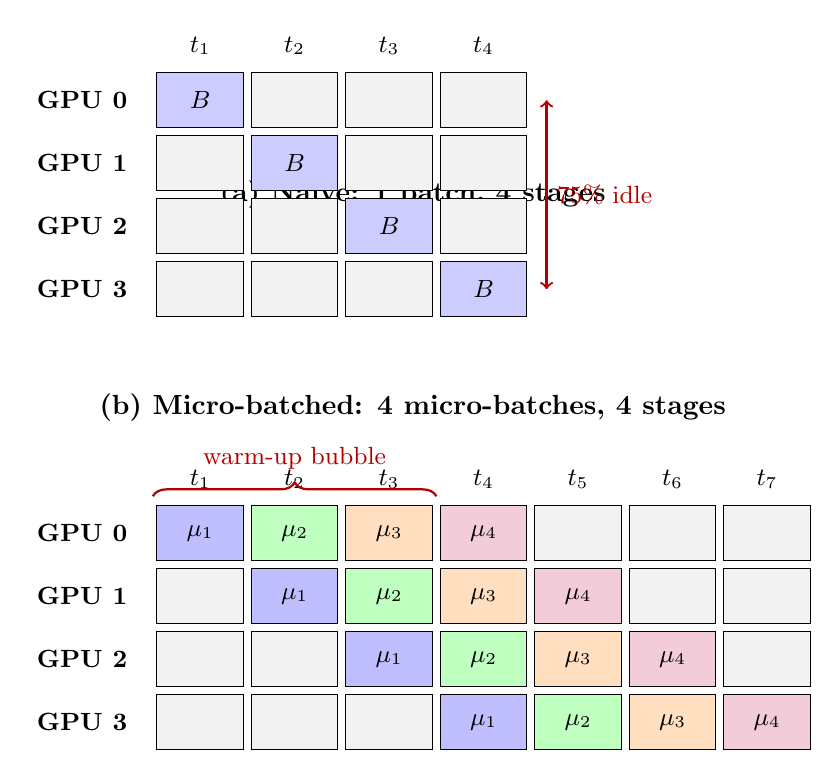
\begin{tikzpicture}[
    cell/.style={minimum width=1.1cm, minimum height=0.7cm, align=center, font=\small},
    active/.style={cell, draw, fill=blue!20},
    idle/.style={cell, draw, fill=gray!10, text=gray!50},
    label/.style={font=\small\bfseries, anchor=east},
    time/.style={font=\small, anchor=south},
]
% Title: Naive (no micro-batching)
\node[font=\bfseries] at (3.3, 1.2) {(a) Na\"ive: 1 batch, 4 stages};

% Stage labels
\node[label] at (-0.2, 0) {GPU 3};
\node[label] at (-0.2, 0.8) {GPU 2};
\node[label] at (-0.2, 1.6) {GPU 1};
\node[label] at (-0.2, 2.4) {GPU 0};

% Time labels (top, manually placed above row for GPU 0)
\foreach \t in {1,2,3,4} {
    \node[time] at ({(\t-1)*1.2+0.6}, 2.85) {$t_{\t}$};
}

% GPU 0: active at t1
\node[active] at (0.6, 2.4) {$B$};
\node[idle]   at (1.8, 2.4) {};
\node[idle]   at (3.0, 2.4) {};
\node[idle]   at (4.2, 2.4) {};
% GPU 1: active at t2
\node[idle]   at (0.6, 1.6) {};
\node[active] at (1.8, 1.6) {$B$};
\node[idle]   at (3.0, 1.6) {};
\node[idle]   at (4.2, 1.6) {};
% GPU 2: active at t3
\node[idle]   at (0.6, 0.8) {};
\node[idle]   at (1.8, 0.8) {};
\node[active] at (3.0, 0.8) {$B$};
\node[idle]   at (4.2, 0.8) {};
% GPU 3: active at t4
\node[idle]   at (0.6, 0) {};
\node[idle]   at (1.8, 0) {};
\node[idle]   at (3.0, 0) {};
\node[active] at (4.2, 0) {$B$};

% Bubble annotation
\draw[<->, thick, red!70!black] (5.0, 0) -- (5.0, 2.4) node[midway, right, font=\small, red!70!black] {75\% idle};

% Title: Micro-batched
\node[font=\bfseries] at (3.3, -1.5) {(b) Micro-batched: 4 micro-batches, 4 stages};

% Offset for second diagram
\begin{scope}[yshift=-5.5cm]
\node[label] at (-0.2, 0) {GPU 3};
\node[label] at (-0.2, 0.8) {GPU 2};
\node[label] at (-0.2, 1.6) {GPU 1};
\node[label] at (-0.2, 2.4) {GPU 0};

\foreach \t in {1,...,7} {
    \node[time] at ({(\t-1)*1.2+0.6}, 2.85) {$t_{\t}$};
}

% Color scheme for micro-batches
% m1=blue, m2=green, m3=orange, m4=purple
\tikzset{
    m1/.style={cell, draw, fill=blue!25},
    m2/.style={cell, draw, fill=green!25},
    m3/.style={cell, draw, fill=orange!25},
    m4/.style={cell, draw, fill=purple!20},
}

% GPU 0
\node[m1] at (0.6, 2.4) {$\mu_1$};
\node[m2] at (1.8, 2.4) {$\mu_2$};
\node[m3] at (3.0, 2.4) {$\mu_3$};
\node[m4] at (4.2, 2.4) {$\mu_4$};
\node[idle] at (5.4, 2.4) {};
\node[idle] at (6.6, 2.4) {};
\node[idle] at (7.8, 2.4) {};

% GPU 1
\node[idle] at (0.6, 1.6) {};
\node[m1] at (1.8, 1.6) {$\mu_1$};
\node[m2] at (3.0, 1.6) {$\mu_2$};
\node[m3] at (4.2, 1.6) {$\mu_3$};
\node[m4] at (5.4, 1.6) {$\mu_4$};
\node[idle] at (6.6, 1.6) {};
\node[idle] at (7.8, 1.6) {};

% GPU 2
\node[idle] at (0.6, 0.8) {};
\node[idle] at (1.8, 0.8) {};
\node[m1] at (3.0, 0.8) {$\mu_1$};
\node[m2] at (4.2, 0.8) {$\mu_2$};
\node[m3] at (5.4, 0.8) {$\mu_3$};
\node[m4] at (6.6, 0.8) {$\mu_4$};
\node[idle] at (7.8, 0.8) {};

% GPU 3
\node[idle] at (0.6, 0) {};
\node[idle] at (1.8, 0) {};
\node[idle] at (3.0, 0) {};
\node[m1] at (4.2, 0) {$\mu_1$};
\node[m2] at (5.4, 0) {$\mu_2$};
\node[m3] at (6.6, 0) {$\mu_3$};
\node[m4] at (7.8, 0) {$\mu_4$};

% Bubble annotation
\draw[decorate, decoration={brace, amplitude=5pt, raise=2pt}, thick, red!70!black]
    (0.0, 2.8) -- (3.6, 2.8) node[midway, above=8pt, font=\small, red!70!black] {warm-up bubble};
\end{scope}
\end{tikzpicture}
\caption{Pipeline bubble with and without micro-batching. (a)~Na\"ive pipeline parallelism with 4 stages: only one GPU is active per time step, wasting 75\% of GPU time. (b)~Micro-batched pipeline with 4 micro-batches ($\mu_1$--$\mu_4$): after the warm-up phase, all GPUs are active simultaneously. Gray cells are idle (bubble); colored cells are active. The bubble fraction drops from $3/4$ to $3/7 \approx 43\%$ with 4 micro-batches, and further decreases as $M$ grows.}
\label{fig:pipeline-bubble}
\end{figure}

\begin{insightbox}
Pipeline parallelism is complementary to tensor parallelism. A common configuration for very large models is TP within a node (using fast NVLink) and PP across nodes (using slower network interconnects). This exploits the communication characteristics of each strategy: TP requires frequent, fine-grained AllReduce operations ($2L$ per forward pass, needing high bandwidth), while PP requires infrequent, coarse-grained point-to-point transfers (one hidden-state tensor per micro-batch per stage boundary). For a hidden dimension of $d = 8192$ in FP16, a single point-to-point transfer is just $8192 \times 2 = 16$\,KB per token---easily handled even over InfiniBand.
\end{insightbox}

\subsection{PP for Inference vs.\ Training}

Pipeline parallelism was originally developed for training, where both the forward and backward passes create complex scheduling challenges (PipeDream, 1F1B schedules). For inference, the situation is simpler: there is only a forward pass, and the primary concern is latency rather than throughput. In inference, PP increases latency by the communication delay at each stage boundary, but it enables serving models that would not fit on a single node. For a LLaMA-405B model requiring 810\,GB of FP16 memory, a configuration of TP=8 within each node and PP=2 across two 8-GPU nodes distributes 810\,GB across 16 GPUs, requiring roughly 51\,GB per GPU---comfortably within the 80\,GB of an A100.

\begin{notebox}
The latency impact of pipeline parallelism during decode is multiplicative with the number of stages. Each decode step must traverse all pipeline stages sequentially. With 4 stages, a decode step that takes 10\,ms on a single GPU takes at least 10\,ms (the computation is the same, just distributed) plus communication overhead. However, the decode computation time itself decreases because each stage holds fewer layers and thus reads fewer weight bytes from HBM. The net effect depends on the relative costs of computation and communication.
\end{notebox}

\begin{whynotbox}{Why not pipeline the decode phase across requests?}
Micro-batching fills the pipeline by feeding multiple micro-batches in quick succession. During prefill, this works naturally: each micro-batch contains a chunk of tokens that can be processed independently. But during decode, each step generates just one token per request and depends on the previous step's output. Could we pipeline decode by staggering \emph{different requests} across pipeline stages?

\textbf{The dependency problem.} In principle, yes: while GPU~1 processes request~A's layers 21--40, GPU~0 could process request~B's layers 1--20. But the benefit is limited because each decode step is extremely fast (the computation per stage is tiny), so the pipeline communication latency at each stage boundary becomes a significant fraction of the stage compute time. With 4 stages and sub-millisecond compute per stage, even microsecond-scale NVLink transfers add meaningful overhead.

\textbf{In practice.} Continuous batching (Section~\ref{sec:distributed:batching}) is the preferred way to keep GPUs busy during decode: instead of pipelining across stages, it batches many requests together so that each stage processes a large batch of tokens simultaneously. This converts the problem from pipeline fill to batch fill, which is far easier to manage.
\end{whynotbox}

Pipeline parallelism and tensor parallelism address how to distribute the model's layers and weight matrices across GPUs. The next challenge is a different kind of efficiency: how to keep those GPUs busy across \emph{time}, by managing the flow of requests into and out of the system.

\section{Continuous Batching}
\label{sec:distributed:batching}

\marginnote{\emph{Continuous batching:} allowing requests to enter and exit the processing batch at any iteration, rather than waiting for the entire batch to complete.}%
Traditional (static) batching groups multiple requests together and processes them as a unit. All requests in a batch are padded to the same sequence length, and the batch is processed through the model as a single matrix operation. The batch is released only when \emph{every} request has finished generating. The problem is twofold:

\begin{enumerate}
\item \textbf{Head-of-line blocking.} If one request generates 10 tokens and another generates 1{,}000, the 10-token request's output is held until the 1{,}000-token request finishes---a 100$\times$ latency penalty.
\item \textbf{Wasted compute.} After a short request finishes, its slot in the batch continues to consume GPU compute (the model processes padding tokens) until the entire batch completes.
\end{enumerate}

\subsection{Iteration-Level Scheduling}

Continuous batching, introduced by the Orca system (Yu et al., 2022), solves both problems by operating at the granularity of individual decode iterations rather than full requests. At each decode step:

\begin{enumerate}
\item \textbf{Evict completed requests.} Any request that emitted a stop token is removed from the batch, and its KV cache blocks are freed.
\item \textbf{Insert new requests.} Any waiting request is added to the batch. Its prompt is prefilled (or, in some implementations, prefill is deferred to a separate phase).
\item \textbf{Decode.} All active requests in the batch advance by one token.
\end{enumerate}

This dramatically improves both throughput and latency. Throughput increases because GPU cycles are never wasted on completed requests---the batch remains full as long as there are waiting requests. Latency improves because short requests are returned immediately upon completion, not blocked by long ones.

\begin{notebox}
Continuous batching interacts with PagedAttention (Chapter~\ref{ch:kvcache}) in a critical way. Because PagedAttention allocates KV cache blocks dynamically from a shared pool, the scheduler can add new requests to the batch as long as free blocks are available---without pre-allocating a fixed maximum cache size per request. This synergy between dynamic batching and dynamic memory management is what makes high-throughput serving practical. Without PagedAttention, the scheduler would need to reserve worst-case cache memory for each request slot, dramatically limiting the batch size.
\end{notebox}

\subsection{Quantifying the Throughput Gain}

Consider a static batch of $B = 32$ requests, where generation lengths are uniformly distributed between 50 and 500 tokens. The expected longest generation is approximately 500 tokens (the maximum). Under static batching, all 32 requests run for 500 iterations, consuming $32 \times 500 = 16{,}000$ GPU-iterations. The useful work is $32 \times 275 = 8{,}800$ GPU-iterations (using the expected generation length of 275). The utilization is $8{,}800 / 16{,}000 = 55\%$.

Under continuous batching, each completed request's slot is immediately refilled. If the arrival rate is sufficient to keep the batch full, utilization approaches 100\%. Moreover, the total number of requests served in the time it takes to generate 500 tokens is not 32---it is approximately $32 \times 500 / 275 \approx 58$ requests, an 81\% throughput improvement over static batching.

\subsection{Prefill-Decode Interference}

\marginnote{Prefill-decode interference is a primary motivation for disaggregated serving (Section~\ref{sec:distributed:disaggregated}).}%
There is a subtlety: when a new request enters the continuous batch, its prompt must be prefilled---a compute-intensive operation that processes all input tokens in parallel. This prefill computation shares the GPU with ongoing decode iterations for other requests. Because prefill has much higher arithmetic intensity than decode, it can delay the decode iterations, causing latency spikes for in-flight requests. This \emph{prefill-decode interference} is one of the key challenges of continuous batching, and a major motivation for disaggregated serving (Section~\ref{sec:distributed:disaggregated}).


\section{Speculative Decoding}
\label{sec:distributed:speculative}

\marginnote{\emph{Speculative decoding:} using a small ``draft'' model to propose multiple tokens, then verifying them in parallel with the large model.}%
Standard autoregressive decoding generates one token per forward pass, which is inherently sequential. Each decode step reads the full model weights from HBM, but performs only enough computation for a single token. Speculative decoding (Leviathan et al., 2023; Chen et al., 2023) breaks this bottleneck by exploiting the gap between the model's arithmetic capacity and its memory bandwidth utilization.

\subsection{The Algorithm}

The procedure has three steps:

\begin{enumerate}
\item \textbf{Draft.} A small, fast \emph{draft model} $M_q$ (e.g., a 1B-parameter variant of the target model) generates $k$ candidate tokens $\hat{t}_1, \hat{t}_2, \ldots, \hat{t}_k$ autoregressively. Because the draft model is small, each step is fast.
\item \textbf{Verify.} The large \emph{target model} $M_p$ processes all $k$ candidates in a single forward pass (as if they were a prompt of length $k$). This produces the target model's probability distributions $p(\cdot \mid t_1, \ldots, t_{i-1})$ for each position $i = 1, \ldots, k$.
\item \textbf{Accept/reject.} For each position $i$ from left to right: the token is accepted with probability $\min(1,\; p(t_i)/q(t_i))$---which means acceptance is certain whenever $q(t_i) \leq p(t_i)$. If rejected, a corrected token is sampled from an adjusted distribution $\text{norm}(\max(0, p - q))$. All subsequent draft tokens are discarded.
\end{enumerate}

\begin{insightbox}
The verification step is mathematically exact: the accept/reject scheme guarantees that the output distribution is \emph{identical} to what the target model would produce alone. Speculative decoding is not an approximation---it is a lossless acceleration technique. The proof relies on the fact that the adjusted sampling distribution at each rejected position exactly compensates for the bias introduced by the draft model.
\end{insightbox}

\subsection{Speedup Analysis}

Let $\alpha$ denote the average acceptance rate---the probability that the target model accepts a draft token. If the draft model generates $k$ candidates and the target model verifies them in one pass, the expected number of tokens generated per verification step is:

\begin{equation}
\label{eq:spec-tokens}
\mathbb{E}[\text{tokens per step}] = \frac{1 - \alpha^{k+1}}{1 - \alpha}
\end{equation}

\noindent For $\alpha = 0.8$ and $k = 5$:

\begin{equation}
\mathbb{E}[\text{tokens per step}] = \frac{1 - 0.8^6}{1 - 0.8} = \frac{1 - 0.262}{0.2} = 3.69 \;\text{tokens}
\end{equation}

If the verification step (one forward pass of the target model on $k$ tokens) takes roughly the same time as $k$ standard decode steps, the speedup is modest. But here is the key insight: during decode, the target model is \emph{memory-bound}. Processing $k$ tokens costs nearly the same wall time as processing 1 token, because the bottleneck is reading the weights from HBM, not the arithmetic. The model weights are read once regardless of whether we compute attention for 1 position or $k$ positions. The speedup is therefore approximately:

\begin{equation}
\label{eq:spec-speedup}
\text{Speedup} \approx \frac{1 - \alpha^{k+1}}{(1 - \alpha)(1 + c)}
\end{equation}

\noindent where $c$ is the relative cost of running the draft model (typically $c \approx 0.05$--$0.1$ for a well-chosen small draft model). With $\alpha = 0.8$, $k = 5$, and $c = 0.07$:

\begin{equation}
\text{Speedup} \approx \frac{3.69}{1.07} \approx 3.4\times
\end{equation}

In practice, speedups of 2--3$\times$ are common for well-matched draft-target pairs. The acceptance rate $\alpha$ depends heavily on the quality of the draft model and the difficulty of the text being generated: predictable code completions achieve higher acceptance rates than creative writing.

\begin{notebox}
\textbf{Draft model selection.} The draft model must share the same vocabulary and tokenizer as the target model. Common choices include: (a) a smaller model from the same family (e.g., LLaMA-1B drafting for LLaMA-70B), (b) a model obtained by pruning or distilling the target, or (c) a simple $n$-gram model or retrieval-based predictor. The trade-off is clear: a better draft model increases $\alpha$ but also increases $c$. Medusa (Cai et al., 2024) takes a different approach, adding lightweight ``heads'' to the target model itself that predict multiple future tokens in parallel, avoiding the need for a separate draft model entirely.
\end{notebox}

\begin{whynotbox}{Why not use a draft model from a different model family?}
The draft model must share the target model's tokenizer and vocabulary. If the draft model uses a different tokenizer, the token IDs in the draft sequence do not correspond to the same tokens in the target model, and the accept/reject scheme---which compares per-token probabilities $p(t_i)$ and $q(t_i)$---becomes meaningless.

\textbf{Beyond vocabulary.} Even with a shared vocabulary, the draft and target models should have similar ``styles'' of prediction. A draft model trained on code may produce poor acceptance rates when the target model generates prose, because the draft's high-confidence predictions diverge from the target's distribution. This is why same-family models (e.g., LLaMA-1B drafting for LLaMA-70B) typically achieve the highest acceptance rates: they were trained on similar data with similar objectives, so their probability distributions are well-aligned.

\textbf{The Medusa alternative.} If finding a compatible draft model is difficult, Medusa sidesteps the issue entirely by attaching lightweight prediction heads directly to the target model's hidden states. These heads are trained to predict future tokens from the same representation, guaranteeing distribution alignment by construction.
\end{whynotbox}

Speculative decoding accelerates the generation loop by producing multiple tokens per forward pass. But it does not address the fundamental tension between the prefill and decode phases---they have different computational profiles and compete for GPU resources. The next section tackles this structural problem head-on.

\section{Disaggregated Serving}
\label{sec:distributed:disaggregated}

\marginnote{\emph{Disaggregated serving:} running prefill and decode on separate GPU pools, independently scaled.}%
The prefill phase (processing the input prompt) and the decode phase (generating tokens one at a time) have fundamentally different computational profiles that are at odds with each other.

\subsection{The Compute Profile Mismatch}

During \textbf{prefill}, the model processes all $n$ input tokens in parallel. The computation is a sequence of large matrix-matrix multiplications ($\mathbf{X} \mathbf{W}$ where $\mathbf{X} \in \mathbb{R}^{n \times d}$), achieving high arithmetic intensity:

\begin{equation}
\label{eq:prefill-intensity}
\text{Arithmetic intensity (prefill)} = \frac{2 \cdot n \cdot P}{2P} = n \;\text{FLOP/byte}
\end{equation}

\noindent For a prompt of $n = 2048$ tokens, the arithmetic intensity is 2048 FLOP/byte---well above the A100's compute-to-bandwidth ratio of 156 FLOP/byte. Prefill is \emph{compute-bound}: the GPU's arithmetic units are the bottleneck, and HBM bandwidth is fully utilized.

During \textbf{decode}, as we computed in Section~\ref{sec:distributed:bottleneck}, the arithmetic intensity is just 1 FLOP/byte. Decode is \emph{memory-bandwidth-bound}: the arithmetic units are almost entirely idle.

\begin{table}[h]
\centering
\begin{tabular}{lcc}
\toprule
\textbf{Property} & \textbf{Prefill} & \textbf{Decode} \\
\midrule
Tokens processed & $n$ (prompt length) & 1 \\
Arithmetic intensity & $n$ FLOP/byte & 1 FLOP/byte \\
Bottleneck & Compute (FLOPS) & Memory bandwidth \\
Batch dimension & Sequence length & Batch size \\
Latency metric & Time-to-first-token & Inter-token latency \\
\bottomrule
\end{tabular}
\caption{The fundamental asymmetry between prefill and decode. Prefill is compute-bound because it processes many tokens at once. Decode is memory-bandwidth-bound because it processes one token at a time.}
\label{tab:prefill-decode}
\end{table}

\subsection{Why Co-location Hurts}

When prefill and decode share the same GPU (as in most serving systems), they interfere destructively:

\begin{enumerate}
\item \textbf{Decode latency spikes.} When a new request's prefill begins, it consumes the GPU's compute resources for tens of milliseconds (for a long prompt). During this time, all in-flight decode requests are stalled. Users see a sudden pause in token generation.
\item \textbf{Resource mismatch.} The optimal GPU for prefill (high FLOPS) may differ from the optimal GPU for decode (high HBM bandwidth). Co-location forces a compromise.
\item \textbf{Scaling inflexibility.} A workload dominated by long prompts needs more prefill capacity. A workload dominated by long generations needs more decode capacity. With co-located serving, you must scale both together.
\end{enumerate}

\subsection{The Disaggregated Architecture}

Disaggregated serving, as implemented in Dynamo, separates prefill and decode onto different GPU pools. The architecture operates in three phases:

\begin{enumerate}
\item \textbf{Prefill.} A prefill worker processes the input prompt, computing the full forward pass and generating the initial KV cache.
\item \textbf{KV cache transfer.} The computed KV cache is transferred from the prefill worker to a decode worker over the network. For a 70B model with GQA (8 KV heads), $d_k = 128$, and a prompt of 2048 tokens, the KV cache size is:
\begin{equation}
\label{eq:kv-transfer}
2 \times L \times n_{\text{kv}} \times d_k \times n \times 2 = 2 \times 80 \times 8 \times 128 \times 2048 \times 2 \approx 671\;\text{MB}
\end{equation}
This must be transferred over the network, typically via RDMA (Remote Direct Memory Access) for GPU-to-GPU transfers.
\item \textbf{Decode.} The decode worker receives the KV cache and generates tokens autoregressively, appending new KV entries at each step.
\end{enumerate}

\marginnote{Dynamo uses NVIDIA's NIXL library for high-performance GPU-to-GPU memory transfers, enabling RDMA-based KV cache transfer between prefill and decode workers without CPU involvement.}%
The KV cache transfer introduces latency---671\,MB at 25\,GB/s (100 Gbps InfiniBand) takes approximately 27\,ms. This transfer cost must be weighed against the interference cost of co-location. For long prompts (large prefill compute) and many concurrent decode requests (where interference is severe), disaggregation provides a net benefit.

\begin{insightbox}
Disaggregated serving is the key architectural insight that distinguishes Dynamo from simpler inference systems. By separating the compute-bound prefill from the memory-bound decode, each phase runs on hardware optimized for its computational profile. The router (Chapter~\ref{ch:kvrouter}) must now make a two-stage decision: first, which prefill worker should process the prompt (optimizing for cache reuse and compute availability), and second, which decode worker should receive the KV cache (optimizing for memory bandwidth availability and load balance). This two-stage routing is fundamentally more complex than single-pool routing, but it enables independent scaling of each phase---a capability that is essential for cost-effective serving of diverse workloads.
\end{insightbox}

\subsection{Independent Scaling}

The power of disaggregation becomes clear when workload characteristics vary. Consider two scenarios:

\textbf{Scenario A: Summarization workload.} Users submit long documents (8K--32K tokens) and request short summaries (100--200 tokens). Prefill dominates. The system needs many prefill workers but few decode workers.

\textbf{Scenario B: Code generation.} Users submit short prompts (100--500 tokens) and request long completions (1K--4K tokens). Decode dominates. The system needs few prefill workers but many decode workers.

With co-located serving, both scenarios require the same number of GPUs (scaled to the dominant phase), wasting resources on the non-dominant phase. With disaggregated serving, the prefill and decode pools scale independently, potentially halving GPU costs for skewed workloads. Dynamo's planner component monitors active prefill tokens and active decode blocks on each worker, dynamically scaling each pool based on current demand.


\section{Putting It All Together}
\label{sec:distributed:together}

These five techniques are not mutually exclusive---they compose. A production deployment of a 405B-parameter model might use:

\begin{itemize}
\item \textbf{Tensor parallelism (TP=8)} within each 8-GPU node, splitting every layer's weight matrices across all 8 GPUs connected by NVLink.
\item \textbf{Pipeline parallelism (PP=4)} across 4 nodes, assigning roughly 32 of the model's 126 layers to each node.
\item \textbf{Continuous batching} to keep the GPU pipeline full by dynamically inserting and evicting requests at each decode iteration.
\item \textbf{Speculative decoding} with a 1B draft model to generate 3--4 tokens per target-model forward pass.
\item \textbf{Disaggregated serving} to separate prefill onto a dedicated pool of high-FLOPS GPUs and decode onto a pool optimized for HBM bandwidth.
\end{itemize}

The total GPU count in this configuration is $8 \times 4 = 32$ GPUs per model replica, with additional GPUs in the disaggregated decode pool. The system collectively provides $32 \times 3.35 = 107$\,TB/s of aggregate HBM bandwidth (H100), enabling decode throughput orders of magnitude beyond what a single GPU can achieve.


\section{Summary}

\begin{itemize}
  \item The \textbf{single-GPU bottleneck} is both memory capacity (a 70B FP16 model needs 140\,GB; an A100 has 80\,GB) and memory bandwidth (decode arithmetic intensity is 1 FLOP/byte, 156$\times$ below the A100's compute-to-bandwidth ratio).
  \item \textbf{Tensor parallelism} splits weight matrices across GPUs for latency reduction: columns of $\mathbf{W}_1$, rows of $\mathbf{W}_2$ in the FFN; attention heads across GPUs. Requires $2L$ AllReduce operations per forward pass, demanding high-bandwidth NVLink interconnects.
  \item \textbf{Pipeline parallelism} assigns layers to different GPUs, with bubble fraction $(N-1)/(N+M-1)$ when using $M$ micro-batches. Requires only point-to-point communication at stage boundaries, making it suitable for cross-node deployment.
  \item \textbf{Continuous batching} allows requests to enter and exit the batch at each iteration, eliminating the head-of-line blocking of static batching. Interacts synergistically with PagedAttention for dynamic KV cache allocation.
  \item \textbf{Speculative decoding} uses a draft model to propose $k$ tokens verified in one target-model pass, achieving 2--3$\times$ speedup without approximation. Exploits the memory-bound nature of decode: verifying $k$ tokens costs nearly the same wall time as generating 1.
  \item \textbf{Disaggregated serving} separates compute-bound prefill from memory-bound decode, enabling independent scaling and eliminating cross-phase interference. Requires KV cache transfer over the network.
\end{itemize}

\bigskip
\begin{center}\rule{0.5\linewidth}{0.4pt}\end{center}
\bigskip

We now have the conceptual tools to understand every major component of Dynamo. The next chapter traces a request end-to-end through the system, showing how these distributed inference techniques are composed into a working architecture.

\bigskip
\noindent\textbf{Check Your Understanding}

\medskip
\noindent\emph{These questions are answerable from this chapter alone.}

\begin{enumerate}
  \item Why is LLM decode memory-bound rather than compute-bound? What is the arithmetic intensity of a single-token decode step?

  \textbf{Answer:} A single-token decode step performs approximately $2P$ FLOPs (one multiply-add per parameter) but must read all $2P$ bytes of model weights (in FP16) from HBM. The arithmetic intensity is therefore $2P / 2P = 1$ FLOP/byte. The A100's compute-to-bandwidth ratio is 156 FLOP/byte, meaning the GPU is 156$\times$ more capable of computation than the memory system can feed it. The GPU's arithmetic units sit mostly idle, waiting for weight data.

  \item Tensor parallelism and pipeline parallelism both distribute a model across GPUs, but they have different communication patterns. Which requires higher interconnect bandwidth, and why?

  \textbf{Answer:} Tensor parallelism requires higher interconnect bandwidth. It performs $2L$ AllReduce operations per forward pass (two per transformer layer: one for attention, one for FFN), each synchronizing all participating GPUs. Pipeline parallelism requires only point-to-point transfers of hidden-state tensors at stage boundaries---one transfer per micro-batch per boundary, with each transfer being just $d \times \text{sizeof(FP16)}$ bytes per token. This is why TP is used within a node (NVLink, 900\,GB/s) and PP is used across nodes (InfiniBand, 25--100\,GB/s).

  \item In the Megatron-LM FFN partitioning scheme, why is $\mathbf{W}_1$ split by columns and $\mathbf{W}_2$ split by rows, rather than the reverse?

  \textbf{Answer:} Splitting $\mathbf{W}_1$ by columns means each GPU computes a complete slice of the hidden representation (a subset of the $d_{\text{ff}}$ dimensions). The nonlinear activation function $\sigma$ can then be applied locally on each GPU without any communication. If $\mathbf{W}_1$ were split by rows instead, each GPU would produce a partial sum of the full hidden vector, requiring an AllReduce \emph{before} applying the activation function---doubling the total communication from 2 AllReduce operations per layer to 4.

  \item Explain why continuous batching improves both throughput and latency compared to static batching.

  \textbf{Answer:} Throughput improves because completed requests are immediately evicted and their slots refilled with new requests, keeping the batch full at all times. Under static batching, completed requests waste GPU cycles until the longest request finishes. Latency improves because short requests are returned as soon as they finish generating, rather than waiting for the longest request in the batch. A 10-token request in a static batch with a 1{,}000-token request waits 1{,}000 iterations; with continuous batching, it waits only 10.

  \item Speculative decoding is described as producing output \emph{identical} to standard decoding. How is this possible if the draft model makes incorrect predictions?

  \textbf{Answer:} The accept/reject scheme ensures mathematical equivalence. When the draft model's prediction is rejected at position $i$, the system does not simply use the target model's top prediction. Instead, it samples from an adjusted distribution $\text{norm}(\max(0, p - q))$ that exactly compensates for the bias introduced by accepting some of the draft model's tokens. This ensures that the overall probability of generating any particular token sequence is identical to sampling directly from the target model. The draft model affects only the \emph{speed}, never the \emph{distribution} of the output.

  \item For a 70B model with 80 layers, 8 KV heads, $d_k = 128$, and a 4096-token prompt, calculate the KV cache size that must be transferred during disaggregated serving.

  \textbf{Answer:} The KV cache stores both keys and values (factor of 2), for each layer (80), for each KV head (8), with dimension $d_k = 128$, for each token (4096), in FP16 (2 bytes): $2 \times 80 \times 8 \times 128 \times 4096 \times 2 = 1{,}342{,}177{,}280$ bytes $\approx 1.34$\,GB. At 25\,GB/s (100 Gbps InfiniBand with RDMA), this transfer takes approximately 54\,ms.

  \item Disaggregated serving introduces a new cost: KV cache transfer between prefill and decode workers. Under what conditions is this trade-off favorable?

  \textbf{Answer:} The trade-off is favorable when the interference cost of co-located prefill and decode exceeds the transfer cost. This occurs when: (a) prompts are long, making prefill compute-intensive and the resulting decode latency spikes severe; (b) many decode requests are in-flight simultaneously, meaning a single prefill delays many users; (c) the network supports high-bandwidth GPU-to-GPU transfers (RDMA/NIXL), keeping transfer latency low. For short prompts with few concurrent users, the transfer overhead may exceed the interference savings, making co-location preferable.

  \item A deployment uses TP=8 within each node and PP=2 across nodes. The model has 80 layers and $d = 8192$. How many AllReduce operations occur per forward pass, and how many point-to-point transfers occur per micro-batch?

  \textbf{Answer:} Each of the 80 layers requires 2 AllReduce operations (one for attention output, one for FFN output), giving $2 \times 80 = 160$ AllReduce operations per forward pass. Each AllReduce involves 8 GPUs within a node via NVLink. For pipeline parallelism with 2 stages, there is 1 stage boundary, requiring 1 point-to-point transfer of the hidden-state tensor per micro-batch (from node 0 to node 1). This transfer is $8192 \times 2 = 16$\,KB per token in the micro-batch, sent over the inter-node network.
\end{enumerate}
